\begin{enumerate}[label=\thesubsection.\arabic*,ref=\thesubsection.\theenumi]
\item 
Find the area between the curves $y=x$ and $y=x^2$.
\\
\solution
\label{chapters/12/8/3/2}
	\begin{figure}[H]
		\centering
 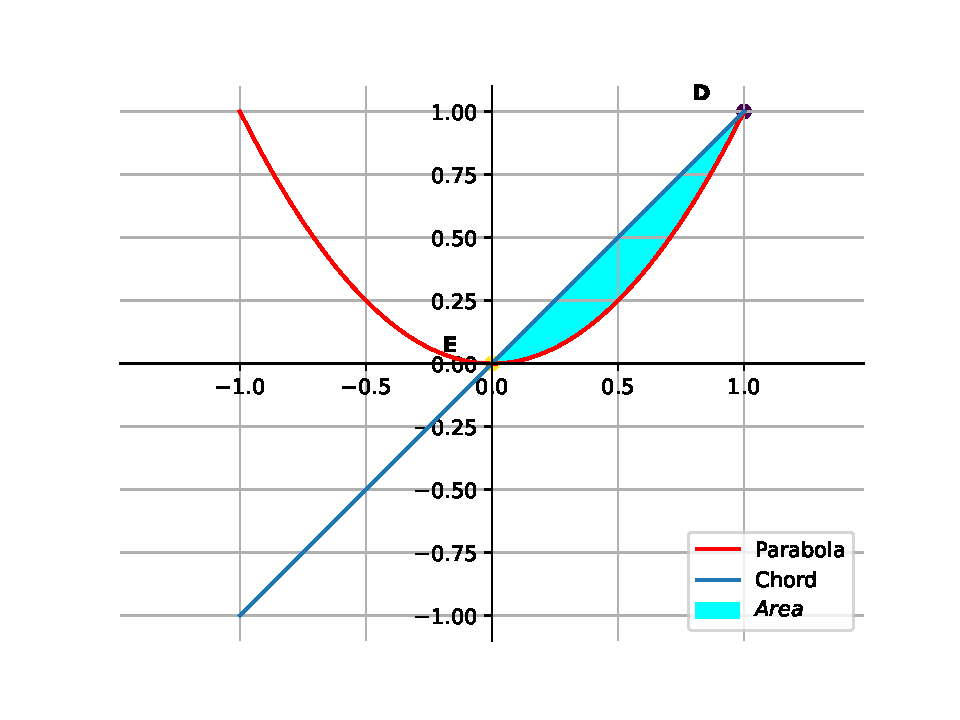
\includegraphics[width=0.75\columnwidth]{chapters/12/8/3/2/figs/fig.pdf}
		\caption{}
		\label{fig:12/8/3/2}
  	\end{figure}
The given curve  can be expressed as a conic with parameters
\begin{align}
	\vec{V} &= \myvec{1 & 0\\0 & 0}, \vec{u} = \myvec{0 \\-\frac{1}{2}}, f = 0
	\end{align}
The given line parameters are
\begin{align}
\vec{h} = \myvec{0 \\0}, \vec{m}=\myvec{1\\1}
\end{align}
Substituting the given parameters in 
\eqref{eq:tangent_roots},
\begin{align}
\vec{x}_1=\myvec{0\\0}, \vec{x}_2=\myvec{1\\1}.
\end{align}
From  
		\figref{fig:12/8/3/2},
the area bounded by the curve $y=x^2$ and line $y=x$ is given by
\begin{align}
	\int_{0}^{1} \brak{x 
	-\frac{x^2}{2}} \,dx = \frac{1}{6}
\end{align}

\item 
Find the area of the region bounded by the curve $y^2=x$ and the lines $x=1$ and $x=4$ and the axis in the first quadrant.
\label{chapters/12/8/1/1}
	\\
	\solution
	\begin{figure}[H]
		\centering
 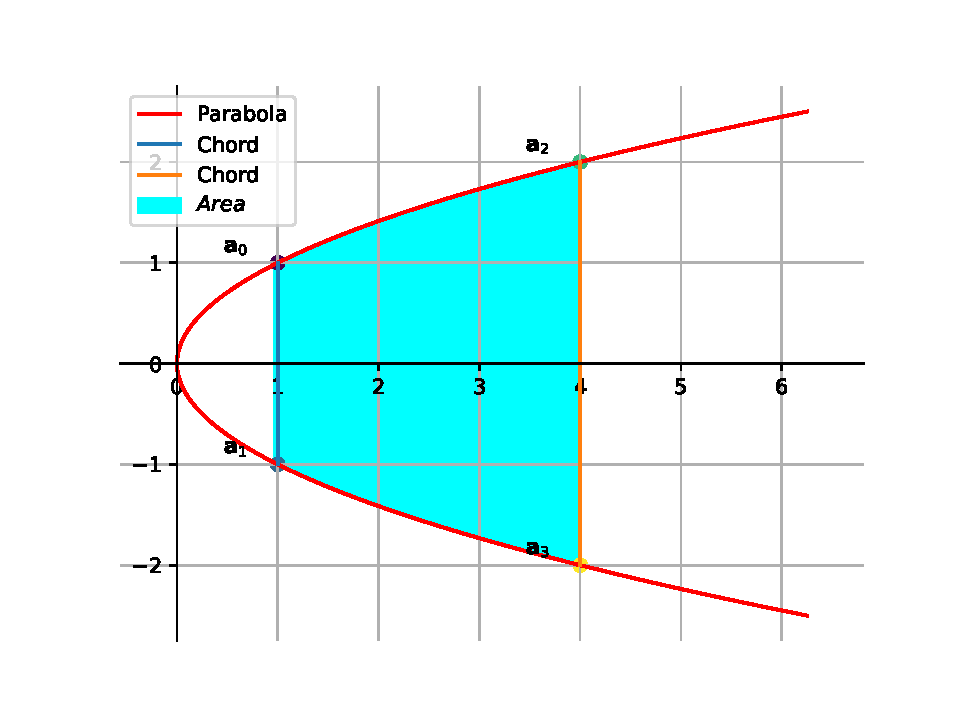
\includegraphics[width=0.75\columnwidth]{chapters/12/8/1/1/figs/fig.pdf}
		\caption{}
		\label{fig:12/8/1/1}
  	\end{figure}

The parameters of the conic are
\begin{align}
	\vec{V} = \myvec{0 & 0\\0 & 1},
	\vec{u} = -\frac{1}{2}\myvec{ 1\\0},
	f = 0
	%\\
\end{align}
\iffalse
The point of intersection of the lines $x=1$ and $x=4$ to the parabola is given by


The points of intersection of the line 
\begin{align}
	L: \quad \vec{x} = \vec{h} + \kappa \vec{m} \quad \kappa \in \mathbf{R}
\label{eq:conic_tangent}
\end{align}
with the conic section are given by
\begin{align}
\vec{x}_i = \vec{h} + \kappa_i \vec{m}
\label{eq:conic_tangent_pts}
\end{align}
%
where
{\tiny
\begin{multline}
\kappa_i = \frac{1}
{
\vec{m}^T\vec{V}\vec{m}
}
\lbrak{-\vec{m}^T\brak{\vec{V}\vec{h}+\vec{u}}}
\\
\pm
\rbrak{\sqrt{
\sbrak{
\vec{m}^T\brak{\vec{V}\vec{h}+\vec{u}}
}^2
-
\brak
{
\vec{h}^T\vec{V}\vec{h} + 2\vec{u}^T\vec{h} +f
}
\brak{\vec{m}^T\vec{V}\vec{m}}
}
}
\label{eq:tangent_roots}
\end{multline}
}
\fi
For the line $x-1=0$, the parameters are  
\begin{align}
	\vec{h}_2=\myvec{1\\0},
	\vec{m}_2=\myvec{0\\1}
\end{align}
Substituting from the above in 
\eqref{eq:tangent_roots},
\begin{align}
\kappa_i=1,-1
\end{align}
yilelding 
the points of intersection 
\begin{align}
	\vec{a}_0=\myvec{1\\1},
	\vec{a}_1=\myvec{1\\-1}
\end{align}
Similarly, 
for the line $x-4=0$ 
\begin{align}
\vec{q_1}=\myvec{4\\0},
\vec{m_1}=\myvec{0\\1}
\end{align}
yielding
\begin{align}
\kappa_i=2,-2
\end{align}
from which, the points of 
intersection are
\begin{align}
\vec{a_3}=\myvec{4\\2},
\vec{a_2}=\myvec{4\\-2}
\end{align}
		See \figref{fig:12/8/1/1}.
Thus, 
the area of the parabola in between the lines $x=1$ and $x=4$ is given by
\begin{align}
\int_{0}^{4} \ \sqrt{x} \,dx-\int_{0}^{1} \ \sqrt{x} \,dx
=14/3
\end{align}

\item 
Find the area of the region bounded by the curve $y^2=9x$ and the lines $x=2$ and $x=4$ and the axis in the first quadrant.
\item Find the area of the region bounded by ${x}^2
= 4{y}$, ${y} = 2$, ${y} = 4$ and the y-axis in the
first quadrant.
\label{chapters/12/8/1/3}
\item Find the area of the region bounded by the ellipse \(\frac{{x}^2}{16}\ + \frac{{y}^2}{9} = 1\)
\label{chapters/12/8/1/4}
\item Find the area of the region bounded by the ellipse \(\frac{{x}^2}{4}\ + \frac{{y}^2}{9} = 1\)
\label{chapters/12/8/1/5}
\item 
		  Find the area of the region in the first quadrant enclosed by the x-axis, line $x=\sqrt{3}y$ and circle $x^2+y^2=4$.
		  \\
		  \solution
\label{chapters/12/8/1/6}
	\begin{figure}[H]
		\centering
 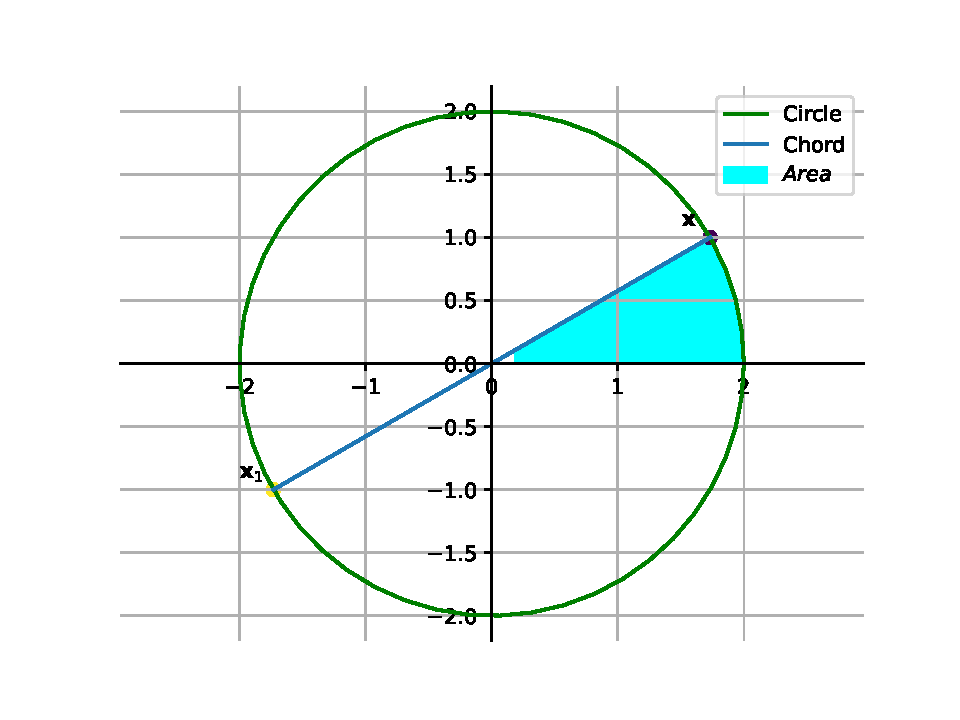
\includegraphics[width=0.75\columnwidth]{chapters/12/8/1/6/figs/fig.pdf} 
		\caption{}
		\label{fig:12/8/1/6}
  	\end{figure}
  From the given information, the parameters of the  circle and line are
                      \begin{align}
			      f= -4, \vec{u}=\vec{0}, \vec{V}=\vec{I}, \vec{m}=\myvec{1 \\ \sqrt{3}}, \vec{h} = \vec{0}
		\label{eq:12/8/1/6}
                    \end{align}                                                                              
Substituting		    the above parameters in  
\eqref{eq:tangent_roots},
	  \begin{align}                                                                               
		  \kappa= \sqrt{3}
	  \end{align}
	  yielding  
the desired point of intersection as                                               
\begin{align}
	\vec{x} = \myvec{\sqrt{3} \\ 1}                               
\end{align}
Note that we have chosen only the point of intersection in the first quadrant as shown in 
		\figref{fig:12/8/1/6}.
From
		\eqref{eq:12/8/1/6},
		the angle between the given line and the $X$ axis is
\begin{align}
	\theta=30\degree
\end{align} 
and
the area of the sector is 
\begin{align}
	{\frac{\theta}{360}}\pi r^2=
	\frac{\pi}{3}
\end{align}

\item 
	Find the area of the smaller part of the circle $x^2+y^2=a^2 $ cut off by the line $x=\frac{a}{\sqrt{2}}$.
\item 
The area between $x = y^2$ and $x = 4$ is divided into two equal parts by the line $x = a$, find the value of a.
\item 
	Find the area of the region bounded by the parabola $y=x^2$ and $y= \abs{x}$.
\label{chapters/12/8/1/9}
\item 
Find the area bounded by the curve $x^2=4y$ and the line $x=4y-2$.
\item Find the area of the region bounded by the curve ${y}^2
= 4{x}$ and the line ${x} = 3$.
\label{chapters/12/8/1/11}
\item Area lying in the first quadrant and bounded by the circle ${x}^2 + {y}^2 = 4$ and the lines ${x} = 0$ and ${x} = 2$ is \rule{1cm}{0.1pt}
\label{chapters/12/8/1/12}
\item Find the area of the region bounded by the curve $y^2 = 4x$, y-axis and the line $y = 3$. 
\label{chapters/12/8/1/13}
\item 
Find the area of the region bounded by the curve $x^2=4y$ and the lines $y=2$ and $y=4$ and the y-axis in the first quadrant.
\item 
	Find the area enclosed by the parabola $4y=3x^2 $ and the line $2y=3x+12$.
\item 
	Find the area of the smaller region bounded by the ellipse $\frac{x^2}{9}+\frac{y^2}{4}=1$
and the line $\frac{x}{3}+\frac{y}{2}=1$.\\
\solution
\label{chapters/12/8/3/8}
	\begin{figure}[H]
		\centering
 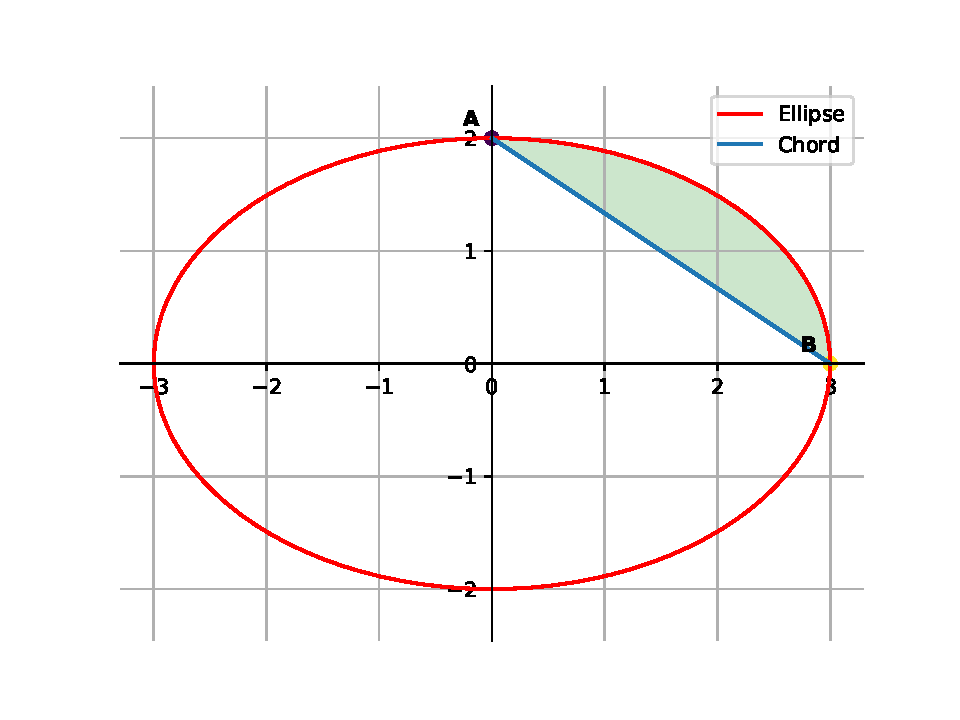
\includegraphics[width=0.75\columnwidth]{chapters/12/8/3/8/figs/fig.pdf}
		\caption{}
		\label{fig:12/8/3/8}
  	\end{figure}
The given ellipse can be expressed as conics with parameters
\begin{align}
\vec{V}=\myvec{
b^2 & 0\\
0 & a^2
},
\vec{u}=0,
f=-(a^2b^2).
\end{align} 
The line parameters are
\begin{align}
\vec{h} &= \myvec{
a\\
0
},
\vec{m} = \myvec{\frac{1}{b} \\ -\frac{1}{a}}.
\end{align}
Substituting the given parameters in \eqref{eq:tangent_roots},
\begin{align}
    \kappa=0,-6
\end{align}
yielding the points of intersection
\begin{align}
    \vec{A}=\myvec{
a\\
0
    },
    \vec{B}=\myvec{
0\\
b
    }.
\end{align}
From 
		\figref{fig:12/8/3/8},
the desired area is
\begin{align}
\int_{0}^{a}\frac{b}{a}\sqrt{a^2-x^2} \,dx 
-\int_{0}^{a} \frac{b}{a}(a-x) \,dx
	= \frac{ab}{2}\brak{\frac{\pi}{2}-1}
	= 3\brak{\frac{\pi}{2}-1}
\end{align}
upon substituting $a=3, b=2$.

\item 
Find the area of the region bounded by the curve $x^2=y$ and the lines $y=x+2$ and the $x$ axis.
\label{chapters/12/8/3/10}
\item 
Find   the area bounded by the curve $y=x|x|, x$-axis and the ordinates $x$=-1 and $x$=1.
\label{chapters/12/8/3/17}
\item 
	Find the area of the region bounded by the curves $y=x^2+2$, $y=x$, $x=0$ and $x=3. $
\label{chapters/12/8/2/3}
\item 
Find the smaller area enclosed by the circle $x^2 + y^2 = 4$ and the line $x + y = 2$. 
\item Find the area of the region bounded by the curves $y^2 = 9x$, $y = 3x$.
\item Find the area of the region bounded by the parabola $y^2 = 2px$, $x^2 = 2py$.
\item Find the area of the region bounded by the curve $y = x^2\text{ and }y = x + 6\text{ and }x = 0$.
\item Find the area of the region bounded by the curve $y^2 = 4x$, $x^2 = 4y$.
\item Find the area of the region included between $y^2 = 9x\text{ and }y =x$
\item Find the area of the region enclosed by the parabola $x^2 = y$ and the line $y = x + 2$
\item Find the area of region bounded by the line $x = 2$ and the parabola $y^2 = 8x$
\item Sketch the region ${(x,0) : y = \sqrt{4 - x^2}}$ and $x$-axis. Find the area of the region using integration.
\item Calculate the area under the curve $y = 2\sqrt{x}$ included between the lines $x = 0\text{ and }x = 1$.
\item Using integration, find the area of the region bounded by the line $2y = 5x + 7$, $x$-axis and the lines $x = 2\text{ and }x =8$.
\item Draw a rough sketch of the curve $y = \sqrt{x - 1}$ in the interval $[1, 5]$. Find the area under the curve and between the lines $x = 1\text{ and }x = 5$.
\item Determine the area under the curve $y = \sqrt{a^2 - x^2}$ included between the lines $x = 0\text{ and }x = a$
\item Find the area of the region bounded by $y = \sqrt{x}\text{ and }y = x$.
\item Find the area enclosed by the curve $y = - x^2$ and the straight line $x + y + 2 = 0$.
\item Find the area bounded by the curve $y = \sqrt{x}$, $x = 2y + 3$ in the first quadrant and $x$-axis.
\item Draw a rough sketch of the region ${(x, y) : y^2 \lessgtr 6ax\text{ and }x^2 + y^2 \lessgtr 16a^2}$.
\item Draw a  rough sketch of the given curve $y =1 + \abs{x + 1}$, $x = -3$, $x = 3$, $y = 0$, and find the area of the region bounded by them, using integration.
\item The area of the region bounded by the curve $x^2 = 4y$ and the straight line $x = 4y - 2$ is
	\rule{1cm}{0.1pt}.
\item The area of the region bounded by the curve $y = \sqrt{16 - x^2}$ and $x$-axis is 
	\rule{1cm}{0.1pt}.
\item Area of the region in the first quadrant enclosed by the $x$-axis, the line $y = x$ and the circle $x^2 + y^2 = 32$ is 
	\rule{1cm}{0.1pt}.
\item The area of the region bounded by parabola $y^2 = x$ and the straight line $2y = x$ is
	\rule{1cm}{0.1pt}.
\item Find the equation of a circle whose centre is (3,1) and which cuts off a chord of length  6 units on the  line $2x-5y+18=0$.
\end{enumerate}
